\section{Organisational plan for the project}
The project was ordered by the sponsor, who also delivers the requirement specification and decides if it is fulfilled or not. All contact with the sponsor and other external parties is handled by the project leader. The project leader shall also plan the work within the group and make sure the group is working towards its common goal. The actual work is not only on the shoulders of the project leader, but on all group members, which play an equal part in the realization of the project. There is also a consultant available for expert help during the course of the project. Figure \ref{organisationsplan} illustrates the organisational structure.

\begin{figure}[H]
  \begin{center}
    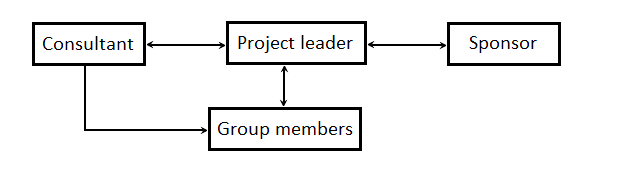
\includegraphics[keepaspectratio=true,width=375px]{grafik/organisationsplan.png}
    \caption{Organizational structure for the project}
    \label{organisationsplan}
  \end{center}
\end{figure}

\subsection{Terms for cooperation within the group}
The group has agreed on the following terms:

\begin{itemize}
\item{All members must be well prepared for meetings.}
\item{Notify the group in time if one can't attend a meeting. In case of illness, this should be reported to the group immediately.}
\item{One shall attend the meetings the group has agreed on.}
\item{If you are unsure of something, you should first seek answers on your own or ask the group. After this external sources may be consulted.}
\item{If a group member doesn't contribute to the project, the rest of the group shall discuss this with the consultant.}
\end{itemize}

\newpage
